\documentclass[]{aiaa-tc}% insert '[draft]' option to show overfull boxes

 \usepackage{varioref}%  smart page, figure, table, and equation referencing
 \usepackage{wrapfig}%   wrap figures/tables in text (i.e., Di Vinci style)
 \usepackage{threeparttable}% tables with footnotes
 \usepackage{dcolumn}%   decimal-aligned tabular math columns
  \newcolumntype{d}{D{.}{.}{-1}}
 \usepackage{nomencl}%   nomenclature generation via makeindex
  \makeglossary
 \usepackage{subfigure}% subcaptions for subfigures
 \usepackage{subfigmat}% matrices of similar subfigures, aka small mulitples
 \usepackage{fancyvrb}%  extended verbatim environments
  \fvset{fontsize=\footnotesize,xleftmargin=2em}
 \usepackage{lettrine}%  dropped capital letter at beginning of paragraph
% \usepackage[dvips]{dropping}% alternative dropped capital package
% \usepackage[colorlinks]{hyperref}%  hyperlinks [must be loaded after dropping]
%\usepackage{makeidx}
\graphicspath{{Images/}}

\usepackage[colorlinks]{hyperref}
%\hypersetup{colorlinks = false}

\usepackage{pdfpages}
\usepackage[ampersand]{easylist}

\usepackage{natbib}
\bibliographystyle{abbrvnat}
\setcitestyle{authoryear,open={(},close={)}}

%AJL SEIT Comment out these two lines for the final submission
%\usepackage{draftwatermark}
%\SetWatermarkFontSize{5cm} \SetWatermarkScale{6} \SetWatermarkText{\textbf{DRAFT-REMOVE}}
\pagestyle{plain}

 \title{Towards Self Driving: Sensing and Learning\\ Interim report}

 \author{
  Michael McDonnell\thanks{CAPT, School of Engineering and Information Technology, ZEIT4901}\
  \\
  {\normalsize\itshape
   UNSW Canberra at ADFA.}\\
  }

 % Data used by 'handcarry' option
 \AIAApapernumber{YEAR-NUMBER}
 \AIAAconference{Conference Name, Date, and Location}
 \AIAAcopyright{\AIAAcopyrightD{YEAR}}

 % Define commands to assure consistent treatment throughout document
 \newcommand{\eqnref}[1]{(\ref{#1})}
 \newcommand{\class}[1]{\texttt{#1}}
 \newcommand{\package}[1]{\texttt{#1}}
 \newcommand{\file}[1]{\texttt{#1}}
 \newcommand{\BibTeX}{\textsc{Bib}\TeX}

%\makeindex

\begin{document}

\maketitle


%\begin{abstract}
%These instructions give you guidelines for preparing your Final Project Summary Report. Use this document as a template if you are using  \LaTeX\ . Otherwise, use this document as an instruction set. The title of this report should be your project title and should NOT contain the word thesis. This section is the abstract, which should concisely summarise your report including the aim, motivations, methodology and observations (or achievements) and conclusions in a single paragraph. Define all symbols used in the abstract. Do not cite references in the abstract. The abstract should be no more than 400 words in length. The footnote on the first page should list your project course. See  \underbar{http://seit.unsw.adfa.edu.au/ojs/index.php/juer} for past examples of final thesis reports, bearing in mind the length requirements may vary.
%\end{abstract}


\tableofcontents
%Anyone know an automated way to do this? Simple as that??!!!!!
%\listoffigures
%\listoftables


%\section*{Nomenclature (examples � include units where appropriate)}
%
%%AJL - COMMENT OUT WHEN YOU WANT TO USE THE AUTOMATIC FILLING OF THE AREA - SEE LATER
%%\printglossary% creates nomenclature section produced by MakeIndex
%\begin{tabbing}
%  XXX \= \kill% this line sets tab stop
%  $J$ \> Jacobian Matrix \\
%  $f$ \> Residual value vector \\
%  $x$ \> Variable value vector \\
%  $F$ \> Force, [N] \\
%  $m$ \> Mass, [kg] \\
%  $\Delta x$ \> Variable displacement vector \\
%  $\alpha$ \> Acceleration, [m/s\textsuperscript{2}] \\[5pt]
%  \textit{Subscript}\\
%  $i$ \> Variable number \\
% \end{tabbing}

\newpage
\section{Introduction} \label{sect:intro}
%\index{}

\lettrine[nindent=0pt]{T}{he} idea of a future where personal transportation is handled by autonomous vehicles is increasingly in the public consciousness however there is a range of challenges that need to be addressed from legal, security and ethical \citep{gmReport} to maturity concerns that out to the 2030s, `autonomous vehicles will be expensive novelties' \citep{vicTransportImplications}. Autonomous driving is not a binary capability however, rather a scale with increasing levels of autonomy. The automation levels identified by the US National Highway Traffic Safety Administration \citep{automationVisionForSafety} outlined in table \ref{t:automationLevels}. While true full automation may be many years off, there is an undeniable increase in the cognitive assistance and partial automation technologies in consumer vehicles. As an example the 2019 Kia Sorento includes active lane keeping assist (lane detection and steering) and adaptive cruise control (autonomous acceleration and braking based off radar distance to leading vehicles) \citep{kia}. 


\begin{table}% no placement specified: defaults to here, top, bottom, page
 \begin{center}
  \caption{automation levels identified by the US National Highway Traffic Safety Administration \citep{automationVisionForSafety}}
  \label{t:automationLevels}
  \begin{tabular}{p{0.1\linewidth}p{0.25\linewidth}p{0.6\linewidth}}
       Level & Classification & Detail\\\hline
        0 &  No Automation & Zero autonomy; the driver performs all driving tasks. \\
       1 &  Driver Assistance & Vehicle is controlled by the driver, but some driving assist features may be included in the vehicle design \\
       2 &  Partial Automation & Vehicle has combined automated functions, like acceleration and steering, but the driver must remain engaged with the driving task and monitor the environment at all times. \\
       3 &  Conditional Automation &   Driver is a necessity, but is not required to monitor the environment. The driver must be ready to take control of the vehicle at all times with notice. \\
      4 &  High Automation &   The vehicle is capable of performing all driving functions under certain conditions. The driver may have the option to control the vehicle. \\
      5 &   Full Automation &   The vehicle is capable of performing all driving functions under all conditions. The driver may have the option to control the vehicle. 
  \end{tabular}
 \end{center}
\end{table}

In order for an autonomous vehicle to navigate effectively there are a few key challenges. The vehicle must have a mechanism to sense the local environment for example lane and road detection as well as transient aspects such as other vehicles and on road obstacles. There are many Computer Vision techniques that can assist in providing an understanding of the environment. Direct techniques such as edge and line detection are widely used however Deep Convolutional Neural Networks have also been shown to be effective for road detection \citep{deepRoadSegmentation}.

In addition to the local area, the vehicle must also have the ability to reconcile navigation data with the current location. A supporting concept to this is that of map matching which calculates out the vehicle location by using the geographical information from sensors such as GPS position and intertial data and the map information from the mapping service \citep{keyTechSelfDriving}. Current high end self driving vehicles require high fidelity 3D maps to operate effectively. Despite this, position localisation improvements have been achieved using a data fusion of GPS and intertial navigation system data \citep{gpsInsFusion} correlating a back lane mark registry (BLMR) supported with CV, GPS and inertial data with map data \citep{lowCostSensorNav} and through use of Kalman filters and LIDAR in more complex environments \citep{robotLIDARSLAM}.

This process of combining data from several sources into a single unified description of a situation is known as data fusion \citep{gpsInsFusion}. Self driving vehicles rely on sensor and data fusion to achieve the four capabilities required of autonomous driving; car navigation system, path planning, environment perception and car control \citep{keyTechSelfDriving}. This project touches on elements of the first three capabilities in order to localise navigation information. The localisation of navigation data will be achieved by the use of GPS position data and computer vision techniques to correlate data from preloaded maps. 

The ability to use computer vision to align GPS positioning with mapping service data will allow greater cognitive assistance in driver included tasks without the requirement for significant prior mapping. As augmented reality technology increases this will also allow driver aides such as navigation routes overlayed onto the visible road. In addition to the cognitive assistance, the ability to localise a navigation route allows the automation of certain tasks such as military field logistics supply lines. A true complete solution will rely on sensor fusion from a suit of complimentary sensors supporting each other and providing redundancy. The idea of local navigation goals has been explored with the use of Open Street Map data and LIDAR for road mapping with promising success \citep{mitLocalNavDriving} however the ability for a single camera system to facilitate navigation data localisation assists in both system redundancy and lowering the financial and technical barriers to implementation.

\subsection{Terminology}

The following abbreviations and definitions are used throughout this report:

\begin{easylist}[itemize]
	& \textbf{Computer Vision (CV)}. Techniques to allow machines to `see'; processing visual images of the world and deriving understanding.
	& \textbf{WORD (abbrev)}. Definition definition
	& \textbf{WORD (abbrev)}. Definition definition
	& \textbf{WORD (abbrev)}. Definition definition
	& \textbf{WORD (abbrev)}. Definition definition
	& \textbf{WORD (abbrev)}. Definition definition
	& \textbf{WORD (abbrev)}. Definition definition
	& \textbf{TODO: External Program, Simulation `tick'}
\end{easylist}

\subsection{Project aim}

The aim of this project is to investigate localising navigation data from a GPS feed to the observed road via a vehicle mounted camera. A subordinate aim as part of this is to develop a simulation that will provide sensor data to an external program for processing. 

GPS route data is held as encoded polylines which represents a road as a series of connected points (nodes) \citep{googleMapPolyline}. The approach for the positional localisation is to use the vehicle GPS position as an approximate input location and detected road features to determine an accurate position of the vehicle and identify the GPS route on forward facing video feed. This sets the conditions for autonomous control of the vehicle based on a programmed nagivation route. 

A subordinate aim to the project is the development of a simulation which provides a sensor data, such as GPS location and video feeds from a simulated vehicle. This simulation will allow both the generation of a large and varied data set for testing as well as allow the ability to provide control feedback for the simulated vehicle based off the processing of the sensor data.

The data flow is anticipated to be as follows:
\begin{easylist}[itemize]
	& Simulated sensor data passed to external program
	& External program processes data:
	&& Road/Lane detection
	&& Curve/Map matching of current GPS area
	&& Reprojection of desired direction onto road image
	& External program returns control data (as applicable) to simulation for next `tick'
\end{easylist}

\subsection{Scope and Deliverables}\label{s:scope}

The scope of the project is deliberately kept constrained initially. This is to focus on the specific problem of localising a navigation route without losing development effort to supporting elements. While the scope is initially narrowly defined it can be extended towards the end of the project as time and opportunity allow.

The scope and deliverables have been identified as follows:
\begin{easylist}[itemize]
	& \textbf{Limitation of road complexity.} There is a requirement for road/lane detection as part of this project (to marry up with the GPS polyline data) however it is not the main focus of the project. Further as the project purely uses the output data of lane detection, it can be considered a `black box' and implementations can be swapped out as more advanced options are identified. The initial limitations on scope of road detection includes:
	&& Limit road detection to easily detectable road surface
	&& Limit roads to single lane
	& \textbf{TODO: OTHER SCOPE?!??!}
	& \textbf{Simulation deliverable requirements.} A core supporting element of this project is the development of the simulation. In addition to providing data for this project the intent is for the simulation to be held as an asset within SEIT for use in subsequent student projects in this area. The basic requirements for the simulation are:
	&& Ability to provide 3D video feed of simulated driving to external program
	&& Support simulated GPS tracking data
	&& Support simulation of GPS route guidance
\end{easylist}

Based on the levels outlined in table \ref{t:automationLevels} the intended level is to level 2 or 3 for cognitive assistance and in automated remote logistics applications such as autonomously traversing known routes in a military field setting to level 4.

\section{TODO: Project management}

\subsection{Project Methodology}
\textbf{TODO: Cut the extra crap from here - just talk about how it flows in general and leave the rest for the current work part}

The initial state of the project consisted of autonomous vehicles as the general area of focus, as a result the first phase of the project was the identification of the `problem area' and narrowing of scope. A broad reading of relevant research and industry articles identified the ability to navigate in arbitrary areas as a candidate problem area and the scope was refined as outlined in section \ref{sect:intro}. 

This project is being undertaken in an area of study that is a new field for the author. As a result the early focus was on developing base competencies in digital image processing and general computer vision. This included a variety of tools and \textbf{TODO: Talk about the analysis of CV options. This included lane detection}

In parallel with the CV competency development, research and experimentation on key technical risk elements of the simulation was conducted. \textbf{TODO: These include.....}

TODO:  Intersection detection, Curve matching (splines etc) and/or Map matching, 

\subsection{TODO: Gantt Chart discussion}

\section{Current work}

The bulk of the initial effort has been developing technical competency within informing disciplines. This includes both the CV technical competency development and addressing the simulation technical risks. Additionally to these aspects, familiarity projects were conducted on neural networks to consolidate the basic theory for potential future use. The projects consisted of developing neuroevolution based solutions for both a physics based ball balancing challenge over the duration of 5 minutes and custom cloned version of the mobile game `flappy bird'. Both solutions used a simple feedforward neural network coded in C\# without the use of any existing libraries with the networks evolving using a custom built genetic algorithm. The CV and simulation aspects are discussed in more detail in the following subsections.

\subsection{Computer Vision}

\textbf{Intent of CV, what are the outcomes (lane detection, intersection detection)}

Before any effective computer vision approaches can be implemented a robust base of understanding of digital image processing is required. \textbf{TODO: Definition of CV, DIP}. In order to develop a robust understanding of DIP concepts study was undertaken using a range of publicly available resources. The main resource used for structured learning was the Spring 2015 offering of ECSE-4540 at Rensselaer Polytechnic Institute by Rich Radke which has the full set of recorded lectures freely available online. Basic algorithms were implemented from first principles in MATLAB which reinforced the internalisation of the concepts. More advanced computer vision concepts were subsequently researched and tested within Python using OpenCV functionality which is discussed further in this section (subsections \ref{s:pythonVc} and \ref{s:openCV}). 

Simple lane detection approaches for straight lanes using the Hough Transform were implemented with varying levels of success. It was noted that the simple approaches suffered when the dashed lane line was faint in comparison with other linear features and when the road was cast in shadow. The final experiment to improve on detection involved lane detection on a video feed using a rolling average of the lower area of interest of the most recent 5 frames of video as input to the lane detection for each frame. The lane detection approach involved identifying straight lines using the Hough Transform of the Canny edge detected area of interest after a low pass filter had been applied. The Hough lines were then chosen based on strength with the strongest line for each angle (side of the lane) chosen. The output consisted of the averaged area of interest with the detected lane lines in red overlayed onto the original frame. An example frame from the video output is included as figure \ref{f:simpleLaneDetectionHough}.

%\begin{figure}[htb]% order of placement preference: here, top, bottom
%	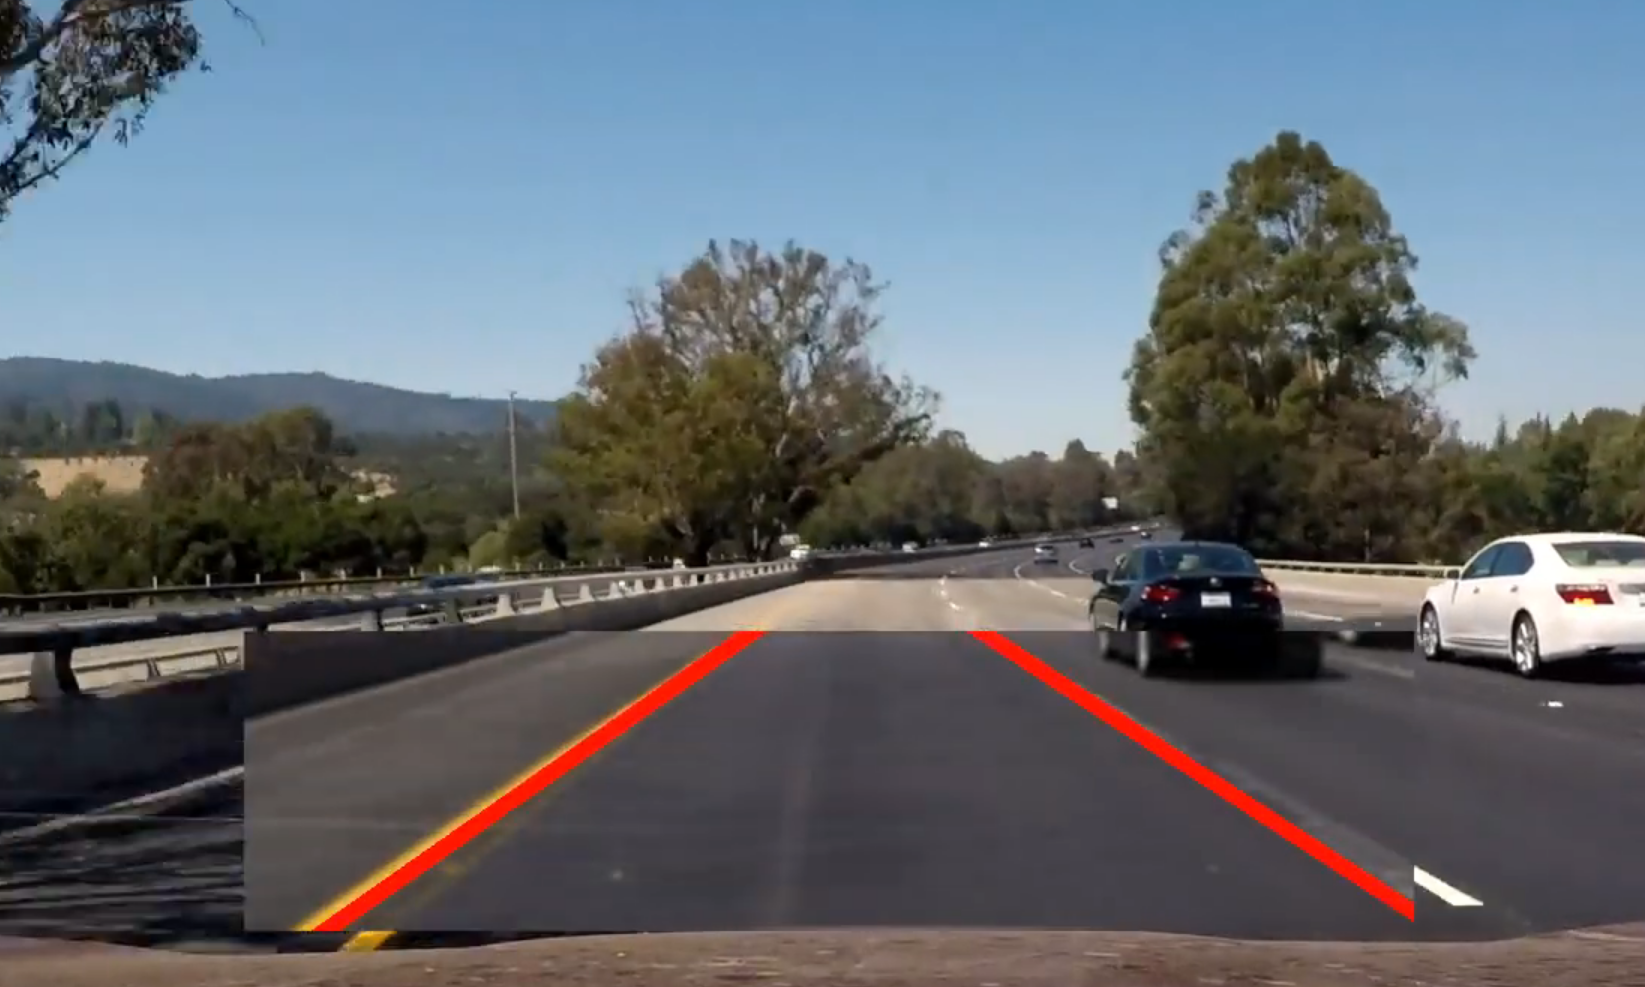
\includegraphics{early_lane_detection_experiment.png}
%	\caption{Still from video feed lane detection experiment}
%	\label{f:simpleLaneDetectionHough}
%\end{figure}

\begin{wrapfigure}{r}{0.5\textwidth} %this figure will be at the right
	\centering
	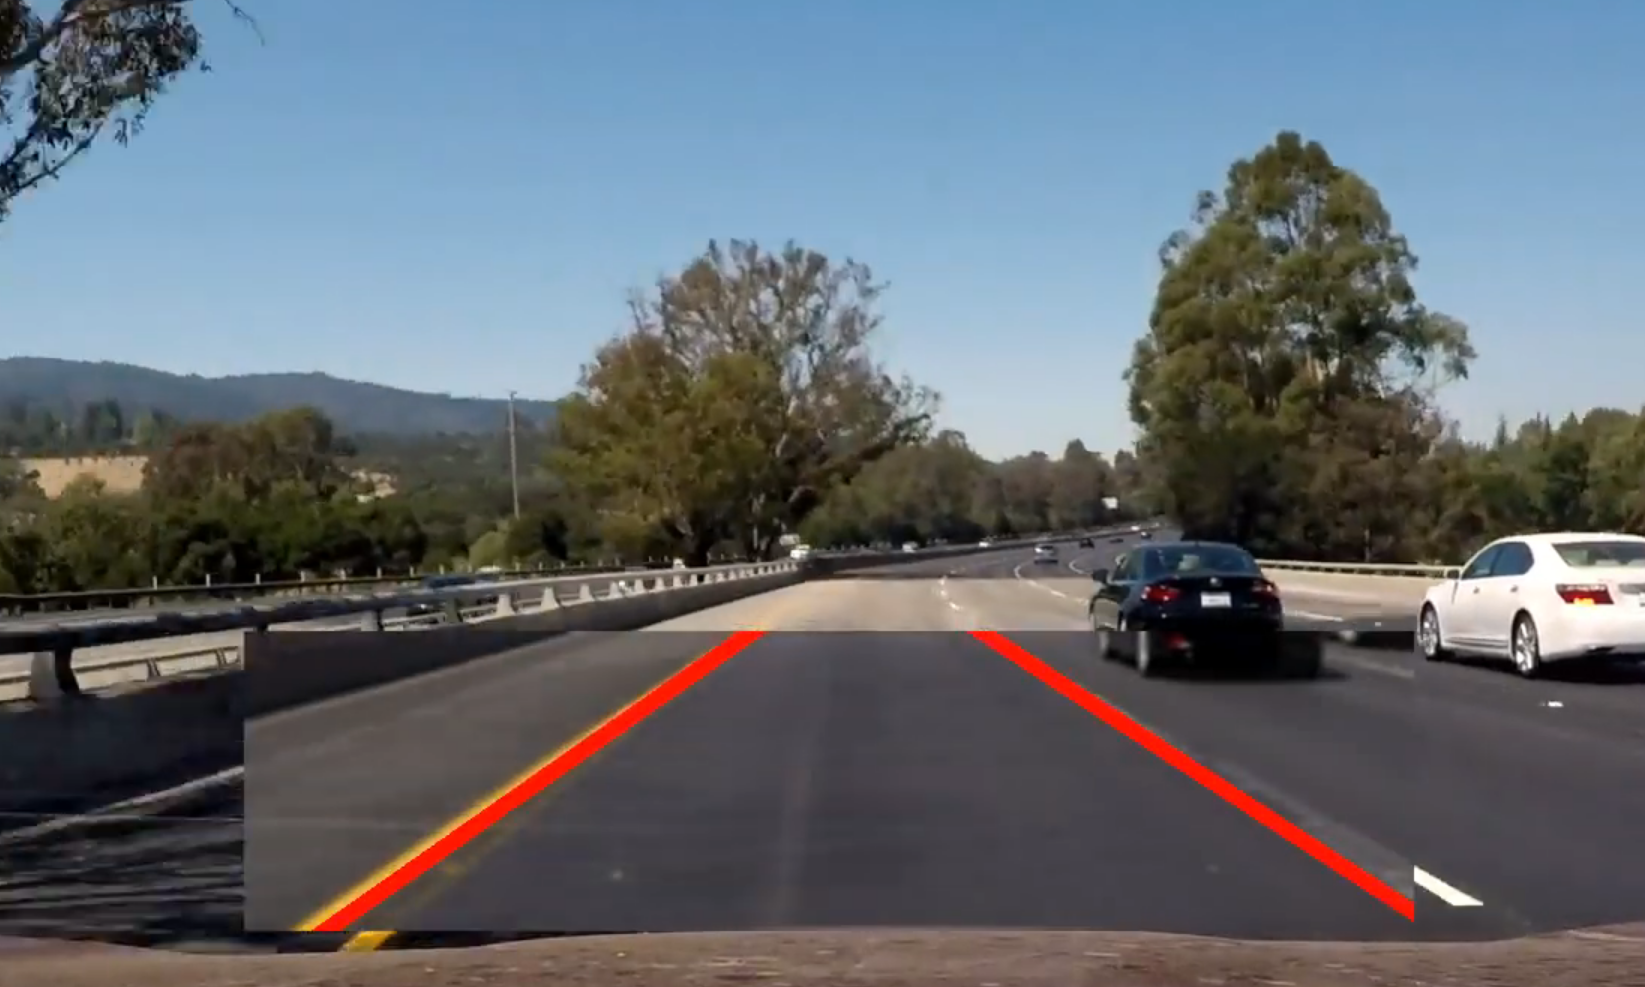
\includegraphics[width=0.5\textwidth, height=0.5\textwidth]{early_lane_detection_experiment.png}
	\caption{Still from video feed lane detection experiment}
	\label{f:simpleLaneDetectionHough}
\end{wrapfigure}

\textbf{THE FLOW OF CV IN LANE DETECTION involves correcting the image for camera lenses before inverse perspective mapping to get a `birds eye view' of the road. From this top down perspective, road/lane analysis can be conducted properly.} An inverse perspective mapping calibration was developed using the interprocess communication implementation discussed in section \ref{s:IPC} \textbf{TODO: THIS ISNT REFERENCING THE FULL SECTION - SHOULD BE III-B-2, NOT JUST 2}. This calibration consists of still image of a checkerboard pattern on the horizontal plane within the simulation taken from the perspective of the camera. Corners of the checkerboard are manually identified in pixel space and the inverse perspective matrix is calculated based on the current old (perspective) and desired new (inverse perspective) positions. Automated identification of checkerboard corners is possible however the simulation camera rotation with reference to the horizontal plane is fixed therefore only a single calibration is required. The input and output of the inverse perspective mapping calibration undertaken is included as figure \ref{f:inverse_perspective_calibration}.

\begin{figure}[htb]% order of placement preference: here, top, bottom
	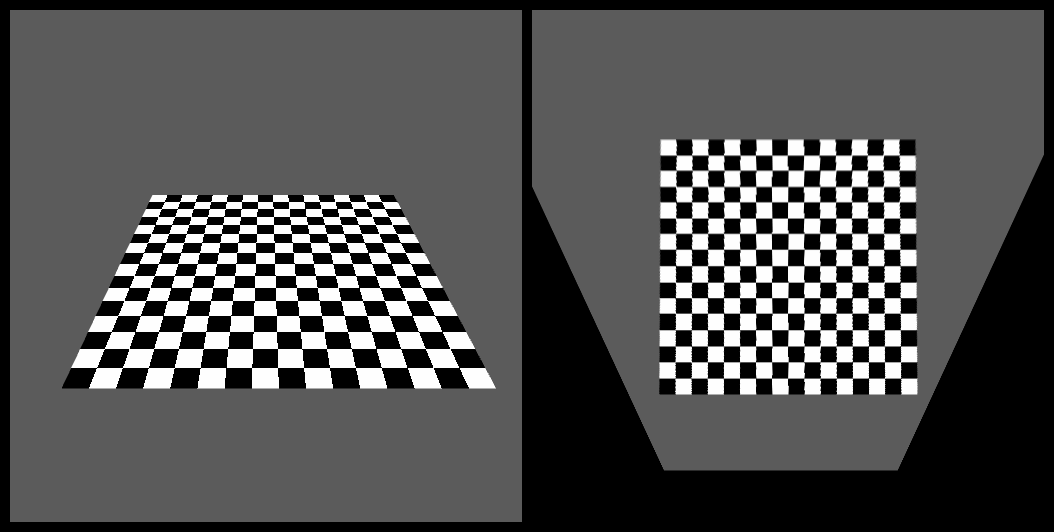
\includegraphics{InversePerspectiveEg.png}
	\caption{Inverse perspective mapping calibration. Original camera feed \textit{(left)} and inverse perspective mapped image \textit{(right)}}
	\label{f:inverse_perspective_calibration}
\end{figure}

Key considerations within the Computer Vision implementation decision process are in the following subsections.

\subsubsection{Open CV}\label{s:openCV}

The DIP theory that was undertaken opened up the possibility to implement the CV functionality from first principles, indeed basic tools such as filtering had already been implemented in MATLAB experiments. The alternative option considered was to use an open source computer vision library called OpenCV. OpenCV has C++, Python, Java and MATLAB interfaces and is widely used in commercial applications in companies such as Google, IBM and Honda \citep{opencvWebsite}. 

While implementing all functions manually has merit for further reinforcement of the basic principles, the decision was made to use the OpenCV library. Rationale for this includes the following: 

\begin{easylist}
	& Efficient high performance vectorised implementations
	& Allows a greater proportion of time to be spent on solving the problem as opposed to implementing known algorithms.
	& Increase familiarity with available tools for future use
\end{easylist}

\subsubsection{Language choice} \label{s:pythonVc}

Given the choice of OpenCV for the CV framework the options considered for the core language were C++ or Python. C++ has the advantage of being `lower level' however the OpenCV Python interface compiles down to the same C++ code so the only performance gains would be in the general program code as opposed to the CV implementations. Simulation engine considerations also played a part, as discussed in section \ref{s:simEngineChoice}, Unreal Engine uses C++ which would allow simulation code to talk directly to the OpenCV interface.

Despite the above advantages, C++ comes with an increased complexity and any speed gains require a robust understanding (and implementation) of memory management. By contrast, Python presents a lower barrier to entry while maintaining the OpenCV C++ vectorised optimisation. In addition, libraries such as numpy within Python present fast vectorised operations for arrays. The descision to use Unity for the simulation engine as discussed in section \ref{s:simEngineChoice} removed the major benefit of the C++ interface thus Python was determined to be the preferred language.

\subsection{Simulation system}

A significant element of the project deliverable is the development of the simulation system to provide sensor outputs. The intent of the simulation is to provide a pipeline of sensor feeds and potentially a \textbf{interface to control a simulated vehicle based off BLAH} with scope of the simulation as discussed in section \ref{s:scope}. \textbf{TODO: ?scope? IPC?} Key elements of the simulation system are discussed in the following subsections.


\subsubsection{Simulation engine} \label{s:simEngineChoice}

Two courses of action were available for the implementation of the simulation engine; a full custom engine or use an existing game engine for the base. For the existing game engine option, Unreal and Unity were both considered. A full custom engine allows fine grain control over the implementation the specific requirements of the simulation however has significant overheads including the implementation of 3D visuals including rendering, texturing and importing of 3D models. It was determined that this represented a very large time commitment for negligable benefit.

Both Unity and Unreal are professional 3D engine used in commercial games and computer graphics applications. They are well established and have a robust set of supporting tools. Specific considerations for each engine are as follows:

\begin{easylist}
	& Unity
	&& Personal experience with workflow; very comfortable
	&& Personal experience with C\# which is used for scripting within the engine
	&& No C\# interface with OpenCV therefore interprocess communication will need to be developed between the OpenCV processing implementation and the simulation engine.
	& Unreal
	&& New, unfamiliar workflow
	&& Lack of familiarity and comfort with C++ which is used for scripting within the engine. `Blueprint' system does allow a visual programming approach although that represents an additional compenancy to be developed
	&& C++ code allows direct interface with OpenCV
\end{easylist}

When considering the above factors and the OpenCV considerations discussed in section \ref{s:openCV}, Unity was chosen due to the ability to `hit the ground running' based on workflow and language familiarity. It was noted that this accepts a large technical risk of IPC implementation however it was deemed to be the preferred option.

\subsubsection{Interprocess Communication (IPC)} \label{s:IPC}

One of the main issues identified with using Python Open CV and the Unity game engine is the ability for simulation data, for example video feeds, to be transferred from Unity to the Python process. This was a significant technical challenge (REF GANTT CHART? HOW LONG WAS BUDGETED). The motivation for fast IPC was to allow real time processing of the simulation data in order to allow for potential control feedback to the simulation. Transferring image data represents a large amount of memory thus has a significant time complexity per simulation `tick'. 

The initial research approach involved investigating the ability to use a static memory buffer that could be written to by Unity and read by Python. Shared memory or memory mapped files do offer this however they add another level of complexity and implementation details are largely for lower level languages and could not be identified in particular for Python. Named pipes were also investigated and, while they represented an improved option, still had many of the technical and implementation complexity issues of the memory mapped approach.

The final solution identified was using TCP via the ZeroMQ middleware. This has implementations for both C\# and Python and is well optimised for speed on localhost (\textbf{TODO: What is localhost}) machines. The speed of this approach is highly dependant on the size of the transferred data \textbf{TODO: GRAPH OF TIME PERFORMANCE OF 64, 128, 256 AND 512....}. The use of this approach requires slower than real time simulation processing which was achieved by dynamic simulation time dilation, discussed in section \ref{sect:timedilation}. This approach allows easy and reliable two way communication which is required for effective feedback between the processes. This is something that would be complicated significantly by memory mapping, requiring multiple memory locations with varying roles. The current solution also offers the ability to expand off a single local machine, for example a hosted simulation with remote processing. While this is well out of scope of this thesis it presents additional flexibility for future development.

Once the IPC approach was confirmed, the data handling pipeline between the Unity (C\#) and Python processes was developed. The final simulation output data structure for video feed is a flattened 3D byte array, consisting of the x and y pixel coordinates and the colour value. The colour is represented by a four element vector of bytes for the Red, Blue, Green and Alpha channels. 

The Python process casts the byte stream as a byte array and reshapes the data to a 3D array. The fourth element of each colour value is removed, resulting in a final data structure consisting of a 2D array of 3 element vectors of bytes which is the required data structure for OpenCV processing operations. 

A simple calibration was established using three coloured cubes (Red, Green and Blue) in Unity to confirm colour channel and axis orientation correctness. A still from the colour image IPC calibration undertaken is included as figure \ref{f:unity_calibration}. \textbf{TODO: Fix image - border? Also shrink and put in/near text}

%\begin{figure}[htb]% order of placement preference: here, top, bottom
% 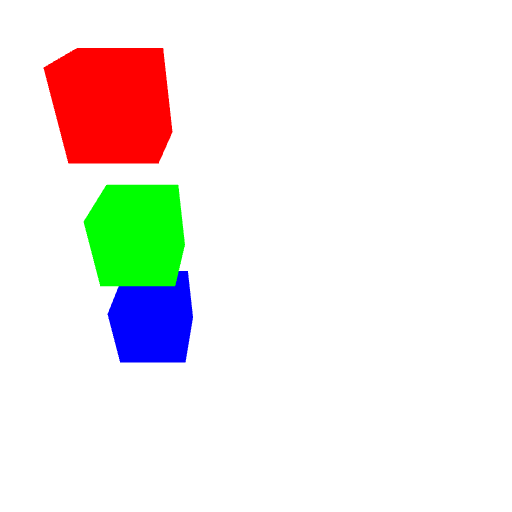
\includegraphics{unity_calibration.png}
% \caption{Still from calibration of colour image IPC pipeline between Unity and Python}
% \label{f:unity_calibration}
%\end{figure}

%[width=50mm,scale=0.5]
\begin{wrapfigure}{r}{0.5\textwidth} %this figure will be at the right
	\centering
	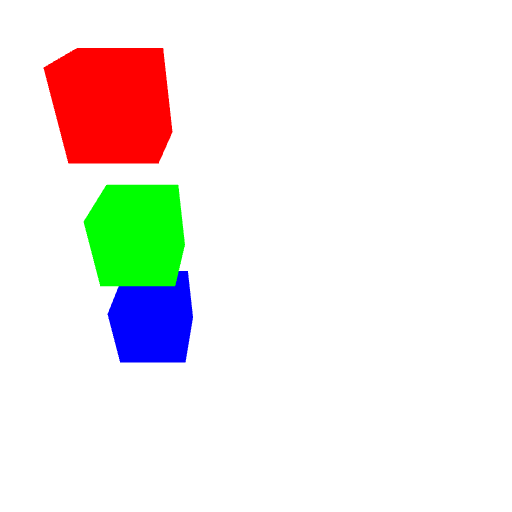
\includegraphics[width=0.5\linewidth, height=0.5\linewidth]{unity_calibration.png}
	\caption{Still from calibration of colour image IPC pipeline between Unity and Python}
	\label{f:unity_calibration}
\end{wrapfigure}

\subsubsection{Simulation time dilation}\label{sect:timedilation}

While the initial design aimed for realtime simulation and processing it was quickly determined that the simulation had a requirement to dynamically scale simulation time. This scaling is based on the external processing in order to ensure the simulation effectiveness regardless of the data processing time requirement and allows both the simulation to be effective on lower end computers and the number of sensors to scale without affecting simulation quality.

The implementation of time dilation involved a simulation controller that runs the simulation for a set time based off the desired sensor processing rate. After this time has elapsed, the sensor data is collated and sent to the external processing program via the IPC process outlined above. On completion of the data processing, the external program sends an acknowledgement in return which triggers the next simulation tick. This has been implemented and tested by sleeping the processing thread for several seconds each tick.

The time dilation was tested using an initial prototype of the simulation in the same manner as the colour calibration discussed previously. Two stills from the output video showing the raw feed and the canny edges is included as figure 

\begin{wrapfigure}{r}{0.75\textwidth} %this figure will be at the right
	\centering
	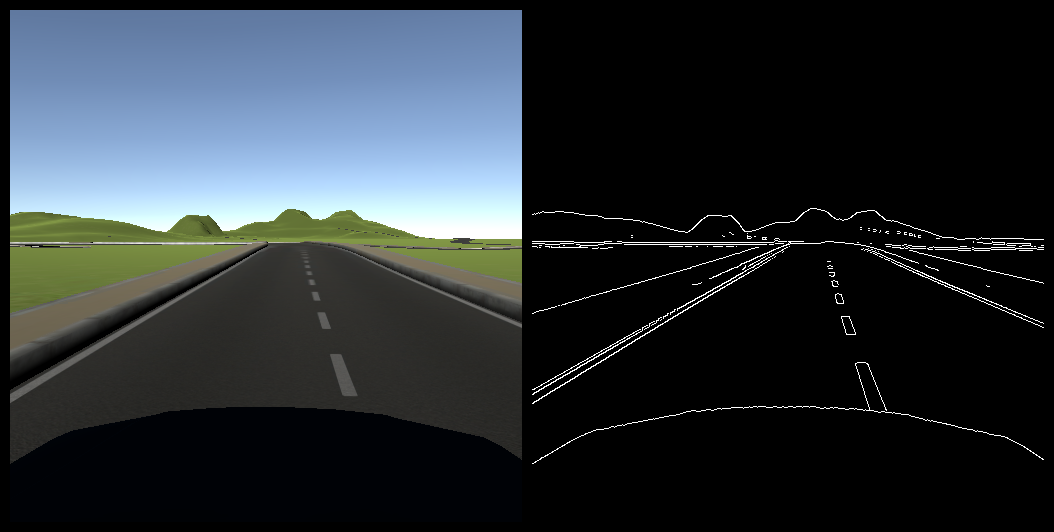
\includegraphics[width=0.75\textwidth, height=0.75\textwidth]{simPrototypeIPC.png}
	\caption{Still from video feed of simulation prototype test. Original camera feed \textit{(left)} and canny edges of feed \textit{(right)}}
	\label{f:simPrototypeIPCTest}
\end{wrapfigure}

\section{TODO: Future work}

The work completed thus far has solved some key technical challenges required \textbf{TODO: }

\subsection{TODO: Road detection}

\subsubsection{TODO: Lane line detection}

Detect the curve of the lane and identify intersections
Curve detection options - sliding window REF LINK %https://www.spiedigitallibrary.org/conference-proceedings-of-spie/0852/0000/Progress-In-Road-Intersection-Detection-For-Autonomous-Vehicle-Navigation/10.1117/12.968232.short?SSO=1

CNN discussion with references?

\subsubsection{TODO: Intersection detection}

\subsection{TODO: GPS Data matching}
Curve matching (splines etc) and/or Map matching, 

\subsection{TODO: Simulation}

Road network
GPS sensor
GPS nav route definition

extensions: Sensor external definitions
%
%\begin{table}[t] % no placement specified: defaults to here, top, bottom, page
% \begin{center}
%  \caption{Expectations for the Assessment of the Final Project Summary Report \
% (Final Project Summary Report is worth 35\% of the course) }
%  \label{t:scheme_marking}
%  \begin{tabular}{|c|} \hline
%\\
%\textbf{Understanding of the topic: (What and why?)} \\\hline
%�	Has the problem been adequately defined? \\
%�	Has a critical review of the relevant literature been performed? \\
%Note the most important references should be included in this report, whereas \\
%extensive literature reviews where appropriate should be confined to the \\
%Appendices or your separate Project Specific Deliverable. \\
%�	Has the relationship between the project and the literature been adequately defined? \\
%�	Has a clear, appropriate and attainable set of aims been identified? \\
%\\
%\textbf{Methodology (How?)}  \\\hline	
%�	Has a logical process been developed to meet the aims? \\
%�	Has this process been justified? \\
%�	Is the methodology appropriate for the scope of the project? \\
%\\
%\textbf{Analysis}	 \\\hline
%�	Has there been an adequate collection of data/information (or efficient design)? \\
%�	Has appropriate and sufficient analysis been performed to reduce it to a useful form? \\
%�	Have the aims been adequately addressed (if not then have valid reasons been given)? \\
%\\
%\textbf{Discussion, conclusions and recommendations:} \\\hline	
%�	Are they meaningful/worthwhile/significant within the scope of the project? \\
%�	Are they appropriate and adequately justified? \\
%\\
%\textbf{Presentation of the project report:}	 \\\hline
%�	Is the document set out clearly and logically? \\
%�	Does the text clearly explain all aspects of the project to even a non-expert? \\
%�	Has appropriate use been made of figures/tables/charts? \\
%�	Has appropriate and accurate use of referencing been made? \\
%\\
%\textbf{Management}	 \\\hline
%�	There is no requirement for an explicit management document, but it may be \\
%appropriate for you to briefly discuss your learnings in terms of expectations \\
%in the context of your project. \\
%\\
% \\\hline
% \end{tabular}
% \end{center}
%\end{table}



%\begin{figure}[htb]% order of placement preference: here, top, bottom
% 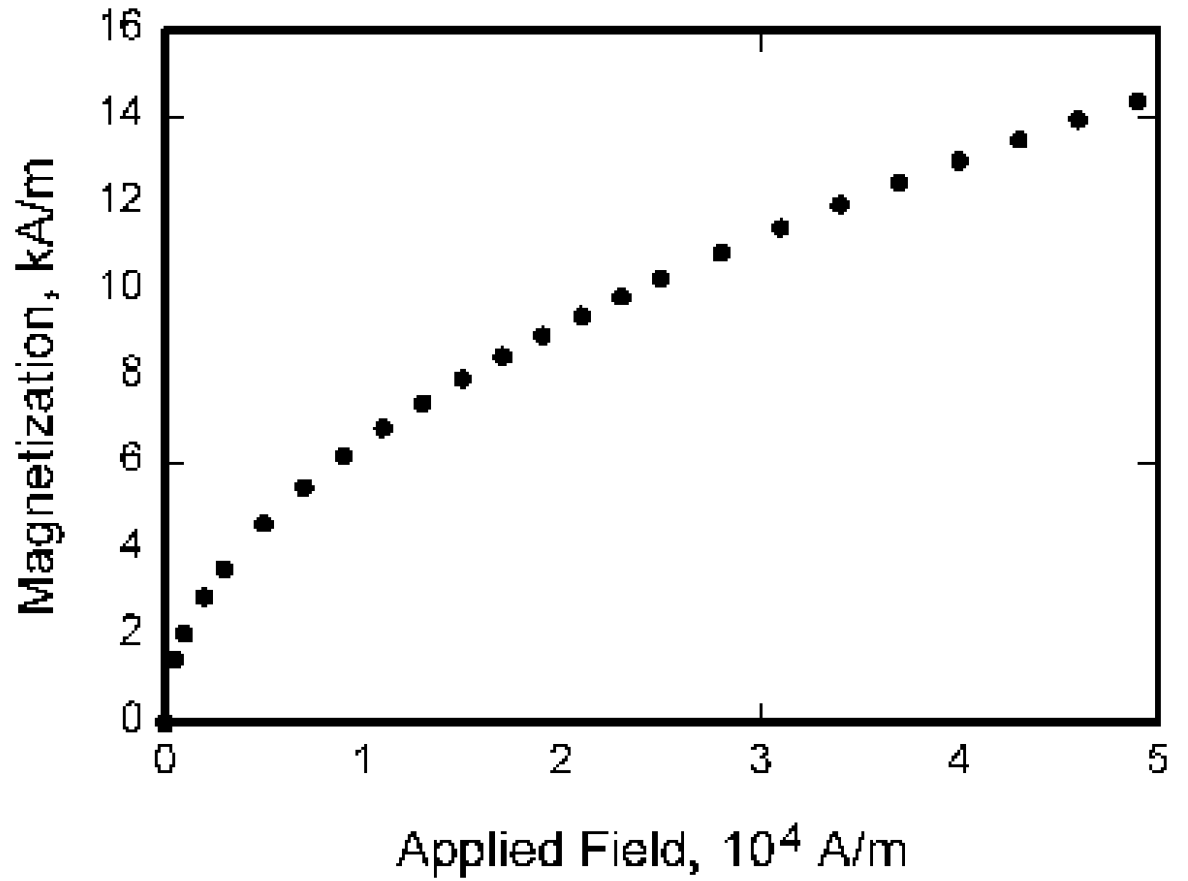
\includegraphics{image_eg.png}
% \caption{Magnetization as a function of applied field, which has
%   borders so thick that they overwhelm the data and for some reason the
%   ordinate label is rotated 90 degrees to make it difficult to
%   read. This figure also demonstrates the dangers of using a bitmap
%   as opposed to a vector image.}
% \label{f:magnetic_field}
%\end{figure}

%Sometimes writing meaningless text can be quiet easy, but other times one is hard pressed to keep the words flowing.\footnote{And sometimes things get carried away in endless detail.}
%
%\begin{table}% no placement specified: defaults to here, top, bottom, page
% \begin{center}
%  \caption{Variable and Fixed Coefficient Runge-Kutta Schemes as a
%           Function of Reynolds Number}
%  \label{t:scheme_comparison}
%  \begin{tabular}{rrr}
%       Re & Vary & Fixed \\\hline
%        1 &  868 & 4,271 \\
%       10 &  422 & 2,736 \\
%       25 &  252 & 1,374 \\
%       50 &  151 &   736 \\
%      100 &  110 &   387 \\
%      500 &   85 &   136 \\
%    1,000 &   77 &   117 \\
%    5,000 &   81 &    98 \\
%   10,000 &   82 &    99
%  \end{tabular}
% \end{center}
%\end{table}

%\subsubsection{Equations, Numbers, Symbols, and Abbreviations}
%Equations are centered and numbered consecutively, with equation numbers in parentheses flush right, as in  Eq.~(\ref{e:function}) that demonstrates some math
%typesetting.

%\begin{equation}
% \label{e:function}
% \int_{0}^{r_{2}} F(r,\varphi) \, dr \, d\varphi =
%    \left[ \sigma r_{2}/(2\mu_{0}) \right] \cdot
%    \int_{0}^{\infty} \exp(-\rho|z_{j}-z_{i}|) \, \lambda^{-1} 
%\end{equation}
%Eq.~(\ref{e:function}) is grand.
%
%
\section{TODO: Conclusions}
The conclusions should summarise the main findings of your thesis project including a brief reference to the supporting evidence and to the initial aims. Note that the Conclusions and Recommendations sections are the last sections of the paper that should be numbered. The acknowledgements and references should be listed without numbers.
This had been a brief example of some of the more advanced options available for \LaTeX\ .
%
%\section{Recommendations}
%This section should discuss and recommend directions for future work that will build on and extend your research and perhaps resolve some of the issues that you have encountered in your work.
%
%\section*{Acknowledgements}
%The Acknowledgements section should be used to briefly thank those individuals or organisations that have assisted you directly in your thesis work whether they be family, friends and colleagues, or technical and academic staff. Note that any external funding source that supported your project should be acknowledged here. 
%
%\section*{Appendices (Separate Document)}
%Appendices may used to archive detailed summaries of data such as images, tables and charts and detailed example calculations such as for the estimation of measurement uncertainty. They may also include design drawings. Raw data, or detailed computer programs and files and extensive design drawings, should not be included. Their archiving should be discussed with your supervisor. Any appendices should be submitted as a SINGLE separate document file if referred to in the main text and be listed in the table of contents at the beginning (Note the use of a separate page numbering scheme).

% If you use MakeIndex
%\printindex


% AJL - UNCOMMENT THIS IS PREFERENCE TO THE ABOVE SECTION
%% produces the bibliography section when processed by BibTeX
\bibliography{InterimReferences}
%\bibliographystyle{aiaa}

\appendix
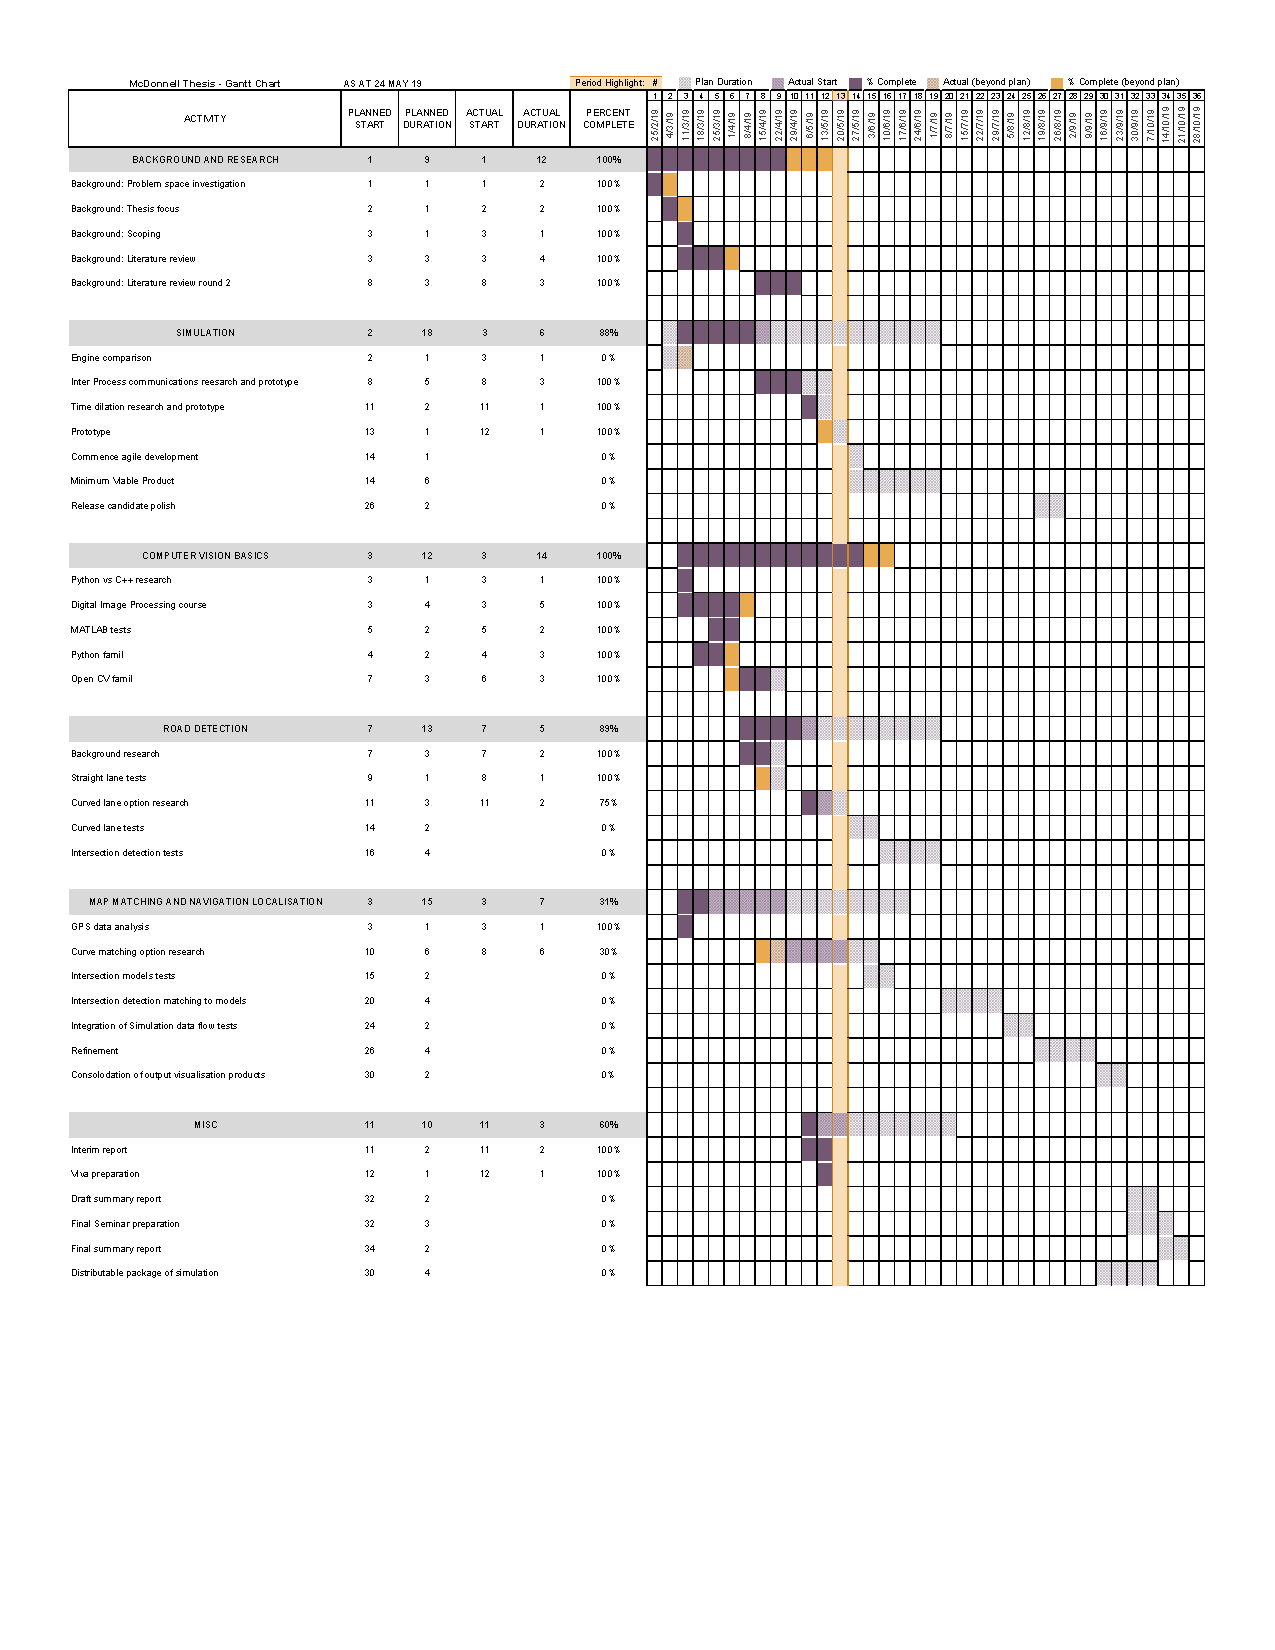
\includepdf[angle=-90,scale=0.9,pages=1,pagecommand=\section{Gantt Chart for Research Project}]{GanttChart.pdf}


\end{document}

